\documentclass{ieee}

\usepackage[latin1]{inputenc}

\usepackage{times}

\usepackage{graphicx}

\usepackage{graphics}

\usepackage[english]{babel}

\title{High Performance Communication System Based on Generic Programming}
                                                                                
\author{Andr� Lu�s Gobbi Sanches\\
  gobbi@lisha.ufsc.br\\
  \and Fernando Roberto Secco\\
  secco@lisha.ufsc.br\\
  \and Ant�nio Augusto Fr�hlich\\
  guto@lisha.ufsc.br\\
  \centerline{Software and Hardware Integration Laboratory - LISHA}\\
  \centerline{Universidade Federal de Santa Catarina - UFSC}\\
}

\begin{document}
          
\maketitle

\thispagestyle{empty}
                                                                      
\begin{abstract}
  This paper presents a high performance communication system
  based on generic programming. The system adapts itself according to
  the protocol being used on communication, simplifying the
  development of libraries. In order to validate the concepts, a MPI
  implementation has been developed and it is compared to a
  traditional implementation - MPICH-GM. It is demonstrated that the
  same functionality and interface can be offered with similar
  performance, but with much less programming effort. That is an
  evidence that the large size of traditional MPI implementations is
  due to the limitations of conventional communication systems.
\end{abstract}

\section{Introduction} 

Traditional communication systems are often organized just like the
OSI protocol stack: each layer provide services to the upper
layers. Each layer may handle the lower ones, but not the upper
layers.

The upcoming of low latency networks and their employ in high
performance computing the traditional communication systems have
proven to be not suited. Their hard layer structure results in higher
latency and processing overhead.  As a result, high performance
communication systems often access the communication hardware directly
and offer the communication system through middleware libraries. This
method is known as OS Bypass.

In the last years, many high performance low level communication
libraries have been developed. All libraries offer similar
functionality, but each has its own programming interface. In order to
enable the development of portable parallel programs, standard
interfaces such as MPI (The Message Passing Interface Standard) have
emerged.  MPI has become the \emph{de facto} standard for low level
communication. Almost every library support its interface, so that MPI
programs are highly portable.

	However, MPI \emph{implementations} are often large and
complex, and building a library that conforms to the standard requires
quite some effort. As an example, the MPI implementation over the GM
low level library for Myrinet networks has 120.000 lines of code,
where 30.000 are not portable \footnote{those numbers were obtained by
analyzing the source code of MPICH-GM}. MPI is often provided as a
middleware library organized in layers, where some are
platform-independent and others are not. This architecture is similar
to the traditional communication system, whose inefficiency was the
reason behind OS Bypass.

	Taking into account the number of lines of code that are
needed to make a library conform to the standard, one could conclude
that are big differences between the low level libraries. But by
analyzing the non-portable code of the implementations, one can
realize that it deals mostly with the message queues and the
operations that manipulates them (registering, receiving and
cancelling) and operating system functionalities (memory management
and DMA). 

	However, MPI programs are not the only ones which need queue
management, and therefore it should not be a responsibility of the
implementation. This resource is required by most applications and
should be provided by the low level libraries.  But this resource is
often provided by middleware, because the queues must be organized by
the MPI protocol header, in order to ensure that no message will ever
be mistaken.

	Those libraries should be generic and support any higher
layers' protocols, and so they do not handle the headers. The queue
system is dependent on the headers, and so the low level libraries do
not handle them.

	However, this design decision enforces the higher level
libraries, or even the applications, to inflate their code with
functionality that are not their responsibility.  Each library must
implement its own queues, that results in duplicate code among the
libraries. In this paper, we show that it is possible to develop a
communication system which handles the higher layers protocol headers
but that is generic, based in recent software engineering techniques.
We also show that this change can greatly reduce the size of a MPI
implementation and other libraries, respecting the interface and
behavior stated by the standard and achieving similar performance. Indeed, we do not provide a middleware library, but just the essence of
MPI: ``The Message Passing \emph{Interface} Standard''.

This paper is organized in this manner: Section 2 describes the message queue system emploied in most MPI implementations. In Section 3 the architecture of a traditional communication system is depicted. In Section 4 the Communication System Based on Generic Programming is presented. A MPI implementation using this communication system is presented in section 5. And Section 6 concludes.

\section{The Message Queue System} \label{sec::queues}

The MPI standard states that the delivery of messages should be
ordered according to the headers of the messages. As a result of this,
most implementations use a queue system where arriving messages are
stored until they are requested by the application. The queue system used
by most implementations has been described by O'Carrol et al
\cite{Carrol:1998}. The set comprises two send queues and two receive queues.

The receive queues are \emph{expected} and \emph{unexpected}. The
\emph{expected} queue is used to store the messages that have already
been requested by the user through the receive calls (immediate or
blocking). The messages have the header that identifies them and the
address of the buffer where the contents should be stored. The
\emph{unexpected} queue is used to store the messages that have
already arrived from the network, but that have not been requested by
the user yet. When a message arrives from the network, a matching
header is searched for in the \emph{expected} queue. If the search is
positive, the content is copied to the buffer of the message and the
related communication is \emph{completed}. If it is negative, the
contents are stored in a temporary buffer and the message is stored in
the \emph{unexpected queue}, as illustrated in Figure \ref{fig:arrival}.
When a receive call is posted, the \emph{unexpected} queue is searched for a matching message. If it is found, the communication is completed. Otherwise, the requested message is stored in the \emph{expected} queue, as illustrated by Figure \ref{fig:recv}.

\begin{figure} \centering
  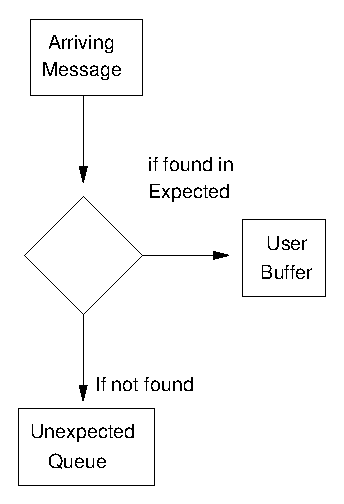
\includegraphics{figures/arrival.eps}
  \label{fig:arrival}
  \caption{Flow of data when a messages arrives}
\end{figure}

\begin{figure} \centering
  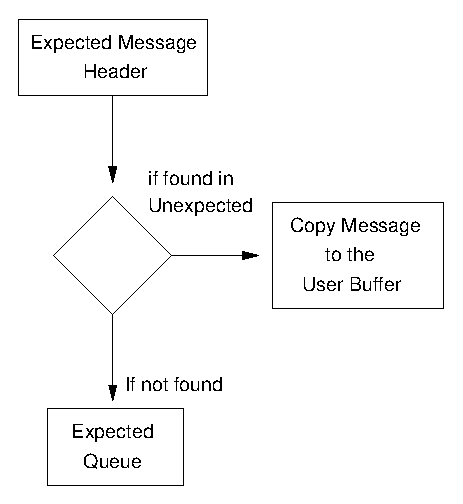
\includegraphics{figures/recv.eps}
  \label{fig:recv}
  \caption{Flow of data on a receive operation}
\end{figure}

The send queues are necessary in order to provide \emph{rendezvous}
communication. When an unexpected message arrives from the network,
a temporary buffer is necessary to store the contents until the receive call is
posted, resulting in an extra memory copy. This memory copy can be a
performance hazard when the message is large. In those cases, only the
header of the message is sent at once, and the contents are kept at
the sender side until they are requested by the receiver. They will be
requested only when a matching receive call is posted, and the user
buffer is already known. Thus, the extra memory copy is avoided. If
the request for a message arrives before the send call is posted, the
contents are sent at once with the header. In order to provided this
kind of communication, two send queues are necessary. 

Those send queues are \emph{requested} and \emph{unrequested}, and
they are analogous to the receive queues. \emph{Requested} store the
requests for messages whose send call has not been posted yet, and
whose contents should be sent at once. \emph{Unrequested} store the
contents of messages whose header has already been sent, but that have
not been requested. When a send operation is called and
\emph{rendezvous} should be used, the \emph{requested} queue is
searched for a matching request. If it is found, the contents are sent
immediately. Otherwise, the contents are stored in the
\emph{unrequested} queue. When a request arrives from the network, the
\emph{unrequested} queue is searched for a matching message. If the
search is positive, the contents are sent. Otherwise, the request is
kept in the \emph{requested} queue. This procedure is illustrated in Figure \ref{fig:send}.

\begin{figure} \centering
  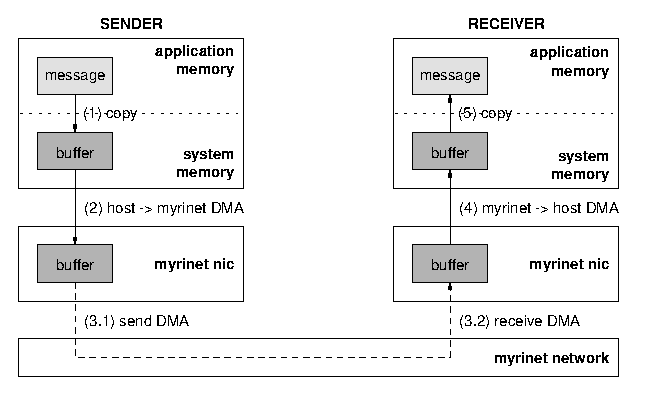
\includegraphics{figures/send.eps}
  \label{fig:send}
  \caption{Flow of data on a send operation}
\end{figure} 

As one can realize, the queue system is important in send or receive
operations. Its handling should be done by the underlying
communication systems, because \emph{ordering} and \emph{rendezvous}
are functionalities that are provided by most message passing
systems. However, since the queues are organized by the headers of the
application protocol (MPI), they are often handled by the MPI
implementation .

\section{Traditional Communication Systems}

	In order to exemplify traditional communication systems, The
	GM message passing system and the MPI implementation based on
	it (MPICH-GM) are going to be described. Those libraries have
	been chosen because they are the combination most used on
	Myrinet networks, which have been used in our
	studies. Firstly, GM will be briefly presented. Secondly, the
	multi-layered architecture of MPICH will be described. At last,
	the layer of MPICH that deals with GM will be described also.

	GM \cite{GM} is the low level message passing system for
	Myrinet network supplied by its manufacturer, Myricom. Its
	design goals include: low CPU overhead, portability, low
	latency and high bandwidth. GM provides reliable ordered
	delivery in the presence of network faults. It bypasses the
	operating system in order to reduce the latency of
	messages. GM provides data link (OSI layer 2) functionality
	through a set of send and receive functions.

	An adaptation of MPICH over GM is also provided. MPICH
	\cite{Gropp:1996:HPI} is a portable MPI implementation. It has
	ports for many low level communication systems. Its
	architecture is organized in three layers: the Channel
	Interface, the Abstract Device Interface (ADI) and the Device
	Independent Layer. The Channel Interface is a set of five
	simple data link functions, that are sufficient to port MPICH
	(but the performance is probably not optimal). The ADI
	provides a set of more than forty functions, that handle MPI
	point-to-point communication, except for data type
	handling. The Device Independent Layer handles collective
	communication, data type handling and any functionality that
	is not based on the communication system. The collective
	operations are based on the point to point functions so that
	they are portable, but one may override their
	implementations.

	Most ports of MPICH start by providing a Channel Interface and
	using a template ADI based on it. The ADI is further
	customized in order to optimize the implementation. The ADI
	handles the message queue system and any functionality that is
	based on it, such as immediate communication. 
	The port of MPICH over GM is just an ADI. The ADI handles the
	queue system, which is organized by the MPI header. When a
	receive function is called, it is registered on the expected
	message queue. When a message arrives from the network, it's
	header is compared to the header of each message in the
	expected queue. When a match is found, the related operation
	is completed. 

	Since the queue system must know the header of the application
	protocol (MPI) it must be handled in the MPI
	implementation. However, that implies that much functionality
	that is shared by most communication system (such as immediate
	communication) must be provided by the implementation, even
	when they are also provided by the lower level libraries. If
	the queue system could be handled by the lower level
	libraries, then most of the functionality of an ADI could be
	handled by them also and a MPI implementation would just be a
	thin layer between two different programming interfaces.

\section{A Communication System Based on Generic Programming}

As presented in the previous sections, most of the functionality of an
ADI is dependent on the message queue system. That functionality must
be provided by the MPI implementations because the lower level
libraries does not handle MPI headers in order to remain generic and
support other protocols as well. In this section, a new communication
system which can manage the queue system is presented.

The proposed communication system is based on a communication proposed
by Fr�hlich for the EPOS operating system \cite{Frohlich:2001}. In
this system, there are 3 main components: \emph{Envelope},
\emph{Communicator} and \emph{Network}. \emph{Envelope} is an
abstraction for the messages, \emph{Communicator} handles transport
layer functionality and \emph{Network} is an abstraction for the
underlying network (Myrinet in our experiments). The system is
family-based \cite{Parnas:1976} and each member of a family has a
different level of functionality. For instance, there are a
\emph{Typed Envelope} for heterogeneous networks and an \emph{Untyped
Envelope} for homogeneous networks. The appropriate \emph{Envelope}
represent the class, so that data conversion is only provided if
needed, but that does not affect any other component of the
system. Each member of the \emph{Communicator} family represents a
different level of transport functionality: \emph{ordered delivery},
\emph{reliable delivery}, etc.

The EPOS communication system is highly configurable, however as
originally proposed by Fr�hlich, it does not handle the upper layer's
protocol headers, and thus cannot handle the queue system. However, we
were able to find that the \emph{Communicator} component can handle
the queues if the system has another abstraction: the \emph{Header}
component.

\subsection{The Header Component}

The communication system requires that a class represents the header
of the application protocol, and that it realizes the \emph{interface}
(abstract class) \emph{Header}. This interface requires that the
operators \verb!==!, \verb!<! and \verb!=! be provided. The operator
\verb!==! verifies if two headers are equal or different, and is used
in order to define if the messages that arrived from the network are
expected or not. The operator \verb!<! defines the ordering of the
message queues, in order to get best performance. The operator
\verb!=! is used for efficient copying of headers.

There is another restriction on \emph{Header} classes: they must be
contiguous. Contiguous objects can be duplicated with simple memory
copies, and therefore are more efficient. This restriction implies
that no header class may contain pointers or references. Headers are
often contiguous thus this obligation is seldom restricts the
protocols which can be used.

\subsection{The Template Envelope}

Since a header identifies a single message, a \verb!header! property
is necessary on the \emph{Envelope} classes. The class of
\verb!header!  must be generic, so any application protocol can be
used. In order to achieve this, the class of \verb!header!  could be
the abstract class \emph{Header} and the actual class could be defined
on instantiation, using polymorphism. However, that would imply in the
use of virtual methods, which would result in bad performance.  Thus,
instead of virtual methods generic programming will be used through
C++ \emph{templates} \cite{Stroustrup:1997}. The class of
\verb!header! is a \emph{class parameter} of \emph{Envelope}.  As a
consequence, the communication system is generic and can be used with
any application protocol, but the code that is generated is identical
to the one we would get if the class was defined directly.  Therefore,
the performance of the system should not be affected.

In order to define an \emph{Envelope} with an specific header, we only
need to instantiate the \emph{template}. For instance, if we need to
define an envelope for MPI messages we could write:

\begin{verbatim}

  typedef Envelope<mpi_header>
          mpi_envelope;

\end{verbatim}

When the \emph{template} is instantiated, the class of \verb!header!
is defined just like if it was defined directly.

Since the \emph{Envelope} is an abstraction of the messages, the
communication operations just have to instantiate an envelope, define
its properties and pass it to a \emph{Communicator} through the
operators \verb!<<! (send) and \verb!>>! (receive). Those operator
return immediately, and the completion of the operations can be
verified through the \verb!complete! property of \emph{Envelope}.

The upper layer must define if \emph{rendezvous} communication should be
used on each message, because each protocol has its own policy. But
the \emph{Communicator} should do the communication, since it handles
the queue system. Thus, the \emph{Envelope} classes also have a
\verb!rendezvous! property which defines if this kind of communication
should be used. Its default value is false, so that libraries which
do not use \emph{rendezvous} may simply ignore this property. 

\subsection{The Template Communicator}

The message queue system must be handled by the \emph{Communicator}
component. The queues are sets of template envelopes that are
identified and ordered by their headers. The four queues described in
section \ref{sec::queues} are necessary: \emph{expected},
\emph{unexpected}, \emph{requested} and \emph{unrequested}. Those
queues are instances of the \emph{Envelope\_queue} class, which has the
header as a \emph{class parameter}.

The queues are properties of the \emph{Communicator}, and thus it
should also has the header as its \emph{class parameter}. This imply
in a restriction: the system can handle only one protocol a time. If
more than one protocol is necessary, the user must disable the queue
management on the \emph{Communicator} and handle them himself. This
restriction is seldom a problem in high performance environment, where
it is common that only a protocol (often MPI) is used at a time.

By being a template, the \emph{Communicator} component can be adapted
to the header of the application protocol and handle the queues,
relieving the upper layers. Any functionality which was handled in the
upper layers because of the queues may be handled by the communication
system. For instance, the immediate communication may be provided by
this system. The immediate receive operation just register the header
of the message in the \emph{expected} queue, and the immediate send
just register the message in the \emph{unrequested} queue if it cannot
be sent. Cancelling a message is just removing it from all the queues
of the system. By having the header as a parameter, the
\emph{Communicator} can provide those operations. A comparison between
the functionalities provided by the presented communication system and
the traditional ones is shown in figure \ref{fig::comparison}.

\begin{figure} \centering
  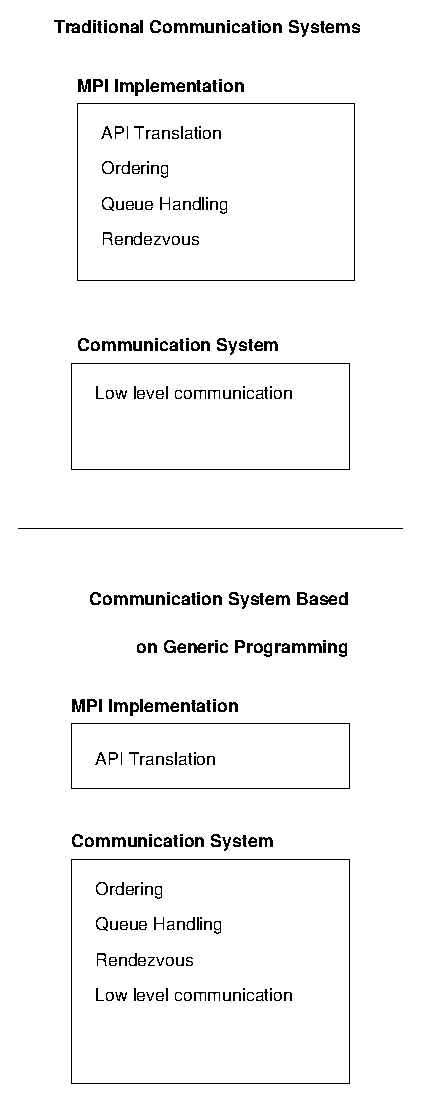
\includegraphics{figures/arch-comp.eps}
  \label{fig::comparison}
  \caption{Comparison between the functionalities of the communication system
  based on generic programming and the traditional ones}
\end{figure}

Besides the complexity of its functions, the interface of the
\emph{Communicator} remains simple. It has only three methods: \verb!<<!
sends an envelope, \verb!>>! receives an envelope and
\verb!check_messages!  verifies if any message has arrived on the
network. When a receive (\verb!>>!) is called, the system compares the
header of the envelope with those on the queues, and when a matching
header (\verb!==!) is found, its content is stored in the buffer
property of the \emph{Envelope}. The \verb!check_messages! method is
called in order to complete immediate operations: it verifies if any
message has arrived from the network device. If a message has arrived
it search the \emph{expected} queue for a matching message. If one
is found, it is completed. Otherwise the arriving message is stored in
the \emph{unexpected} queue.

\section{A Thin MPI Implementation}

In the previous section a communication system based on generic
programming was presented. In order to validate the system a MPI
implementation has been developed over it. Since most of the
functionality is handled by the communication system, MPI has been
implemented as a thin layer. In fact, the implementation was so
smaller and simpler than the traditional ones that the effort required
to develop it entirely was smaller than just adapting another portable
implementation, such as MPICH \cite{Gropp:1996:HPI}.

In this paper only the implementation of the MPI point to point
operations is described. The collective operations are implemented
over the point to point ones and thus they do not depend directly on
the underlying communication system (MPICH handles the collective
communication in the Device Independent Layer).

MPI offers four communication modes: \emph{standard}, \emph{buffered},
\emph{synchronous} and \emph{ready}. They differ only in the use of
\emph{rendezvous}. If the mode is \emph{standard} or \emph{buffered},
\emph{rendezvous} is used only for long messages. If it is
\emph{ready}, it is never used and if it is \emph{synchronous}, it is
always used. This behavior is suggested by the MPI standard
\cite{MPI_1_1}. The property \emph{rendezvous} of the envelope is set
if this kind of communication should be used, and the
\emph{Communicator} will proceed accordingly.

For each communication mode, there are an immediate and a blocking
functions. Since the \emph{Communicator} operators return immediately,
the immediate functions are already supported: they just have to register the
related operation on the queues. The blocking functions do the same
and call \verb!check_messages! in a loop. They return when the
operation is completed (the \verb!complete! property of the envelope
is \verb!true!).

\subsection{The MPI Header}

The MPI standard states that four fields identify a message:

\begin{itemize}
  \item{context;}
  \item{source;}
  \item{destination;}
  \item{tag.}
\end{itemize}

Those four fields compose the \emph{header} of a MPI message, which is
represented by the \verb!mpi_header! class. This class realizes the
\emph{Header} interface, and thus can be used as a class parameter for
the \emph{Envelope} classes. The MPI standard also specifies that
there are two \emph{wild card} values for the properties:
\verb!MPI_ANY_SOURCE! for \verb!source! and \verb!MPI_ANY_TAG! for
\verb!tag!, which define that those properties should not been taken
into account when headers are compared. The operator \verb!==! is used
to compare two headers, so it is aware of the
\verb!wild cards!. Through the class \verb!mpi_header!, the MPI
protocol can be used with the communication system based on generic
programming.

\emph{Message Sending}

In order to send a message, the implementation instantiates an
\emph{Envelope} and passes it to a \emph{Communicator} through the
\verb!<<! operator. The following code is the implementation of the
\verb!MPI_Send! function and is presented in order to illustrate the
simplicity of the implementation.

\begin{verbatim}
int MPI_Send(void *buf, int count
  MPI_Datatype datatype,
  int dest, int tag,
  MPI_Comm comm) {

  Envelope<mpi_header> message(
    mpi_header(comm, MPI_rank,
      dest, tag),
    buf, count, rank2node_id(dest));

  return ((*epos_comm) << message);
}
\end{verbatim}

\subsection{Message Receipt}

The receive operation is similar to the send one. A \emph{Envelope} is
instantiated and initialized with a header that identifies the
expected message and the buffer that should store the contents. The
\emph{Envelope} is passed to a \emph{Communicator} through the
\verb!>>! operator. If the operation is immediate, the \emph{Envelope}
will be stored in the \emph{expected} queue. It will be completed when
the message arrive from the network and the \verb!check_messages!
method of the \emph{Communicator} is called. The \verb!MPI_Wait! and
\verb!MPI_Test! functions test the \verb!complete! property of
the \emph{Envelope} to verify if the operation is complete. If the
function is blocking, then \verb!MPI_Wait! is called just after the
operator \verb!>>!. The implementation of the \verb!MPI_Recv! function
is listed in the following code:

\begin{verbatim}
typedef Envelope<mpi_header>
  *MPI_Request;
const MPI_Request MPI_REQUEST_NULL = 0;

int MPI_Recv(void *buf, int const count,
  MPI_Datatype const datatype,
  int const source, int const tag,
  MPI_Comm const comm,
  MPI_Status * const status) {

  message_t message(
    mpi_header(comm, source, MPI_rank,
      tag),
    buf, count, rank2node_id(source));

  MPI_Request request(&message);

  (*epos_comm) >> message;

  MPI_Wait(&request, status);

  return 0;
}

int MPI_Wait(MPI_Request *request,
  MPI_Status *status) {

  if (*request==MPI_REQUEST_NULL)
    return 0;
  while (!(*request)->complete)
    epos_comm->check_messages();

  set_status(status, *request, 0);
  free_request(*request);

  return 0;
}
\end{verbatim}

\subsection{Comparison}

The advantages of the communication system based on generic
programming can be seen by analyzing the source code of the MPI
implementation. No queue handling is done, and the implementation just
does its job: it translates one API to another. This MPI
implementation is thin because it does not do the job of the
communication system. The ADI of MPICH over GM has more than 30.000
lines of code. The implementation that has been presented has less
than 2.000 lines, and offers exactly the same functionality and
interface.

In figure 2 a performance comparison between MPICH
over GM and the presented MPI implementation is shown. The figure
shows the latency of messages from size 1 to 4096 bytes. The
performance was similar on both implementations, proving that the
flexible architecture of the communication system based on generic
programming does not implies in performance overhead.

However, the code size generated for the presented implementation is
quite smaller. Linking a simple MPI ping-pong program against
our implementation generated a 20KB binary and linking the same code
with MPICH-GM generated a 400KB binary with the same
functionality.

\begin{figure}
  \label{fig::linux_comp}
  \caption{Latency comparison}
  \include{linux_comp}
\end{figure}

\section{Conclusion}

Traditional communication systems are organized according to rigid
architectures, where each layer may handle only the lower layers'
protocols, but not the upper layers'. Since they cannot handle the
upper layer's protocol they cannot manage the queues, and thus some of
the complexity of communication is taken care by middleware libraries
or even by the applications.

A high performance communication system based on generic programming
is presented on this paper. The system is implemented using C++
\emph{templates} which has the application protocol's header as a
class parameter. With this feature, the message queues which are
organized by the header, can be handled by the communication
system. As a result, many communication functionalities that are
dependent on the queues, such as \emph{rendezvous} and immediate
communication, can be offered by the communication system. Therefore,
it plays exactly the role of this kind of system: relieves the upper
layers and the applications from communication code.

This communication system has a limitation: since the
\emph{Communicator} adapts itself to the protocol of the upper layer,
it requires that only one protocol be used at a time. This limitation
is seldom a restriction on high performance environments, where often
only one protocol (often MPI) is used at a time. This is specially the
case when the EPOS operating system is being used, since it is
designed for dedicated systems.

A MPI implementation over this communication system has also been
developed. Thanks to the advanced resources and the simple interface
of the system, the implementation require little effort and few lines of
code. In fact, developing an entire implementation was easier and
faster than just adapting an already existent portable
implementation, thus demonstrating that the presented communication
system has advantages over the conventional ones. The point-to-point
communication functions have very few code: just enable the required
resources and translate from the MPI interfaces to the systems'
one. Therefore, MPI has been implemented just as its essence: ``The
Message Passing \emph{\bf Interface} Standard''.


\bibliographystyle{ieee}

\bibliography{../bib/mpi}

\end{document} % LocalWords: middleware de hlich Medeiros Augusto nio sec
